\documentclass{article}

\usepackage{../preamble}
\standalonetrue

\pagestyle{fancy}
\fancyhf{}
\rhead{Section \thesection}
\lhead{PHYS 304 Lecture 10}
\rfoot{Page \thepage}


\title{PHYS 304 Lecture 10}
\author{Ashtan Mistal}
\date{!!!}

\begin{document}

\ifstandalone
\maketitle
\fi

\graphicspath{{./Lecture10/}}

\section{Review of key points from last lecture}

Although the harmonic wave solutions of the TISE for a free particle, $e^{i k x}$ are not normalizable, and hence the states $e^{i\left(k x-\frac{E}{h} t\right)}$, are not technically stationary state solutions of the full SE, more importantly, any valid wavefunction at $t=0, \Psi(x, 0)$, can still be expanded as a sum over all of the eigen functions of the TISE having a real eigen value. In contrast to the examples we solved involving bounded potentials $V(x)$, where the expansion involved a sum over discrete eigen functions labelled by some integer index $n$, in this case where the eigen energies of the TISE are continuous for $E>0$, the expansion is in terms of an integral over the wavevector associated with each eigen energy, $k=\frac{\sqrt{2 m E}}{\hbar} .$ This should be no surprise, as the expansion $\Psi(x, 0)=$ $\frac{1}{\sqrt{2 \pi}} \int_{-\infty}^{\infty} \phi(k) e^{i k x} d k$, is precisely the Fourier Transform of $\Psi(x, 0)$.

Equally important is that the basic algorithm for finding the full solution of the $\mathrm{SE}, \Psi(x, t)$, knowing $\Psi(x, 0)=\frac{1}{\sqrt{2 \pi}} \int_{-\infty}^{\infty} \phi(k) e^{i k x} d k$, is the same: $\Psi(x, t)=\frac{1}{\sqrt{2 \pi}} \int_{-\infty}^{\infty} \phi(k) e^{i\left(k x-\frac{E}{h} t\right)} d k$

We went through a detailed example where $\Psi(x, 0)$ was chosen to have a real Gaussian form consistent with a probability distribution localized to a range $\sigma$ about some position $x_{0}$ at $t=$ 0 . The full solution for $\Psi(x, t)$ then had a probability distribution in time that stayed centered at $x_{0}$, and remained Gaussian in form, but with a standard deviation that increased monotonically and non-linearly as time progressed. Physically, a stationary, localized free particle will "spread out" or "disperse" as time evolves.

For an electron, if it was localized to start with to an atomic lengthscale, it would disperse extremely rapidly, doubling in extent in a matter of femtoseconds.
For an electron, if it was localized to start with to a laboratory scale, it would remain essentially unchanged for hours.

We further showed that if the purely real, Gaussian shaped $\Psi(x, 0)$ was simply multiplied by $e^{i k_{0} x}$, the full solution for $\Psi(x, t)$ obtained using a Taylor expansion to simplify the Fourierintegral-over- $k$ form of $\Psi(x, t)$, corresponded to a localized wavepacket of Gaussian shape (the amplitude), modulating a harmonic (carrier function), $e^{i k_{0} x}$. The Gaussian envelop moved with a "group velocity" $v_{g}=\frac{h k}{m}$, with the carrier harmonic moving through the envelope with a phase velocity $v_{p}=\frac{\hbar k}{2 m}$. From the Taylor expansion, the group velocity of the wavepacket is given by the derivative of the dispersion relation for the component waves: $v_{g}=\frac{h k}{m}=\frac{d \omega}{d k}=\frac{d E / \hbar}{d k}$. Note that this is the expectation value of the velocity of the particle in the "fudged" harmonic state $e^{i\left(k_{0} x-\frac{E}{h} t\right)}$ we tried to normalize by assuming the universe has a finite extent.

Putting all of these observations together, one concludes that although it is convenient to think of the fudged harmonic wave $e^{i\left(k_{0} x-\frac{E}{\hbar} t\right)}$ as an effective "stationary state" of a free particle, technically it is better to consider a wavepacket state delocalized over macroscopic scales, formed from a continuous sum of harmonic waves with wavevectors clustered very near $k_{0}$, as the closest thing to a free-particle "stationary state". The group velocity of the wavepacket, related to the rate that the amplitude envelope moves, corresponds to the expectation value of the momentum operator in such a state, while the phase velocity dictates the speed of the underlying phase front of the wave.

\section{Today: Finite Potential Well}

TODO: Copy from handwritten notes

\subsection{Activity 1}

Consider first the case of a potential step, as shown below. You should now be gaining some intuition for how wavefunctions "work", with many of their properties akin to classical waves (on a string, or in a pond, or laser beams etc.)
1. Just using words, what would happen to a particle with energy $>0$ propagating to the right in region I (a Step Potential wavepacket), when it reaches $x=0$ ? As an analogy, think of a laser beam, with region I being air (refractive index 1) and region II being a semi-infinite piece of glass, with some refractive index $n>1$.
2. How would you go about solving the TISE for $E>0$ for a particle in this potential environment?

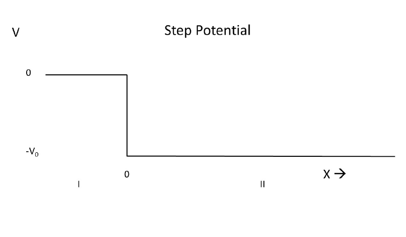
\includegraphics[width = 0.6 \textwidth]{Lecture10/1.png}

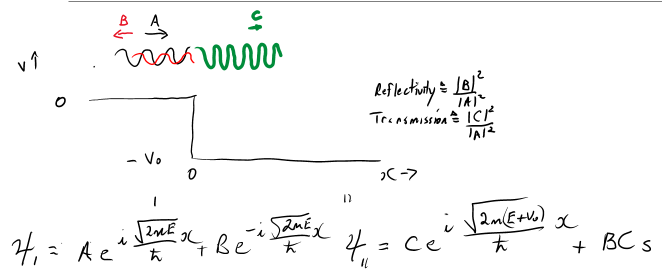
\includegraphics[width = 0.8 \textwidth]{Lecture10/2.png}

\subsection{Activity 2}

What would be the difference if the “incident electron” with E>0 approached from the right?

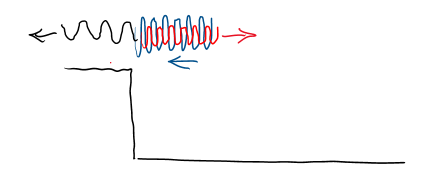
\includegraphics[width = 0.4 \textwidth]{Lecture10/3.png}

Thus there will be two distinct solutions of the TISE for a given E>0, labelled by “right propagating” and “left propagating”.  In contrast to the free electron, the two states are not trivially related.

\subsection{Activity 3}

What about if you repeat for the full finite square well potential, E>0, electron incident from the left?

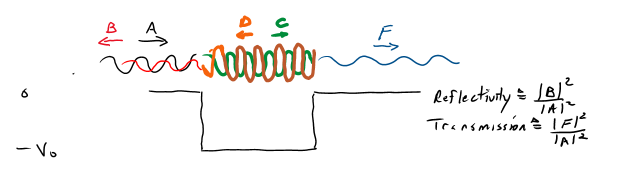
\includegraphics[width = 0.8 \textwidth]{Lecture10/4.png}

$$\frac{F}{A}=\frac{e^{-2 i k a}}{\cos (2 l a)-i \frac{k^{2}+l^{2}}{2 k l} \sin (2 l a)} \quad k=\frac{\sqrt{2 m E}}{h}, l=\frac{\sqrt{2 m\left(E+V_{0}\right)}}{h} \quad T^{-1}=1+\frac{V_{0}^{2}}{4 E\left(E+V_{0}\right)} \sin ^{2}\left(\frac{2 a}{\hbar} \sqrt{2 m\left(E+V_{0}\right)}\right)$$

You should be able to convince yourselves that there are enough BCs to solve for the necessary unknowns.

\subsection{Activity 4}

Compare the energy values at which there is no “reflected” wave included in the eigen state, with those of the infinite square well solution obtained earlier in the course.  Interpret this result. \footnote{From slides: Connect to anti-reflection coating from low index glass on top of higher index substrate (180 degree phase of reflection from front surface, 0 degree phase of reflection from back surface, so if round trip propagation phase. 
}

See below:

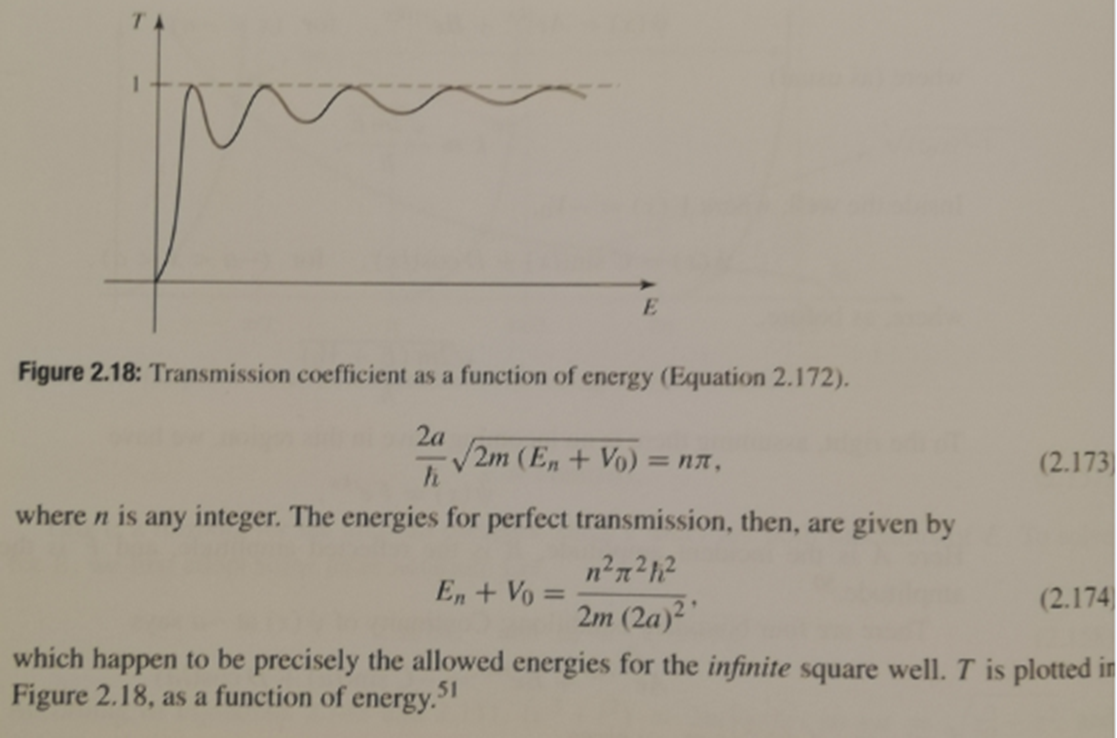
\includegraphics[width = 0.9 \textwidth]{Lecture10/5.png}







\end{document}